\documentclass{article}
\title{pyvb: Variational Bayesian Networks in python}
\author{James Hensman, Mike Dewar}
\date{\today}


\usepackage{amsmath}
\usepackage{amsfonts}
\usepackage{graphicx}
\begin{document}
\maketitle

\section{Bayesian Networks}
\section{Variational Bayes}
\section{A Gaussian Node}


\section{Operations}
\subsection{Addition}
\subsection{Multiplication}
Consider the updating of a node $A$, with parent nodes $\mu_A$ and $\Lambda_A$.  A has a child node $C$, with co-parents $\Lambda_C$ and (through multipication) $B$.  The situation is shown in figure \ref{fig:mult_markov}
note that the nodes $B$,$C$,$\mu_A$ and $\Lambda_A$ form the Markov blanket (is this the correct term? I think so) of A, and so no other information is required for the update - even if the network stretched for many nodes in any direction.  

We're assuming the $A$ is right-multiplied by $B$, i.e. %we have $p(C) = \mathcal{N}(C | AB, \Lambda_C)$.  The log joint probability is:

\begin{equation}
-2 \log p(.) = 
\end{equation}


\begin{figure}
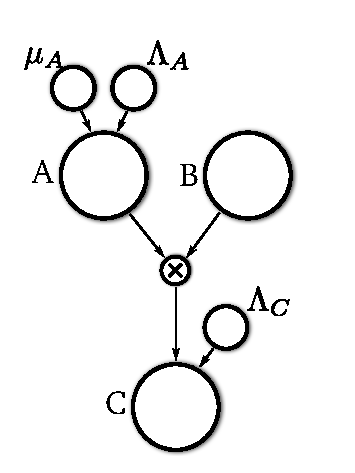
\includegraphics{images/mult_markov}
\label{fig:mult_markov}
\caption{The markov blanket o the node A}
\end{figure}

\subsection{Hstacking}

\section{Precision Nodes}
\section{Gamma}
\section{Diagonal Gamma}
\section{Wishart}


\section{Appendix}
\subsection{The Gaussian Distribution}
\subsection{The Gamma Distribution}
\subsection{The Wishart Distribution}

\end{document}